\subsection{Investimento fase di Analisi}

\subsubsection{Divisione oraria}
La seguente tabella rappresenta la distribuzione oraria dei ruoli per ogni componente del gruppo:
{

	\rowcolors{2}{\evenRowColor}{\oddRowColor}
\renewcommand{\arraystretch}{2}
\begin{longtable}[h!] { C{3.3cm} C{1cm} C{1cm} C{1cm} C{1cm} C{1cm} C{1cm} C{2cm}}
\caption{Tabella della divisione oraria di Analisi}	\\
\rowcolor{\primaryColor}

\textcolor{\secondaryColor}{\textbf{Membro del gruppo}} & 
\textcolor{\secondaryColor}{\textbf{RE}} & 
\textcolor{\secondaryColor}{\textbf{AM}} & 
\textcolor{\secondaryColor}{\textbf{AN}} & 
\textcolor{\secondaryColor}{\textbf{PT}} & 
\textcolor{\secondaryColor}{\textbf{PR}} & 
\textcolor{\secondaryColor}{\textbf{VE}} & 
\textcolor{\secondaryColor}{\textbf{Ore complessive}}\\	
\endhead
\AW{}                     &  - &  - &  14 & - & - & 14 & 28 \\
\AT{}                     &  - &  10 & 10 & - & - & 8 & 28 \\
\AD{}                     &  - &  - &  14 & - & - & 15 & 29 \\
\EC{}                     &  - &  10 & 10 & - & - & 8 & 27 \\
\EM{}                     &  17 &  - & 7 & - & - & 8 & 32 \\
\FP{}                     &  - &  15 & 10 & - & - & 9 & 34 \\
\GG{}                     & 18 &  - &  7 & - & - & 8 & 33 \\
\textbf{Ore totali ruolo} & 35 & 35 & 71 & - & - & 70 & 211 \\

\end{longtable}
}
% Responsabile color=blue, Amministratore color=yellow, Analista color=red, Progettista color=green, Programmatore color=grigetto, Verificatore color=orange  [ybar, fill=] blue, yellow, red, green, grigetto, orange
Il preventivo delle ore da investire per ciascun componente del gruppo per ogni ruolo viene rappresentata nel seguente istogramma:\\
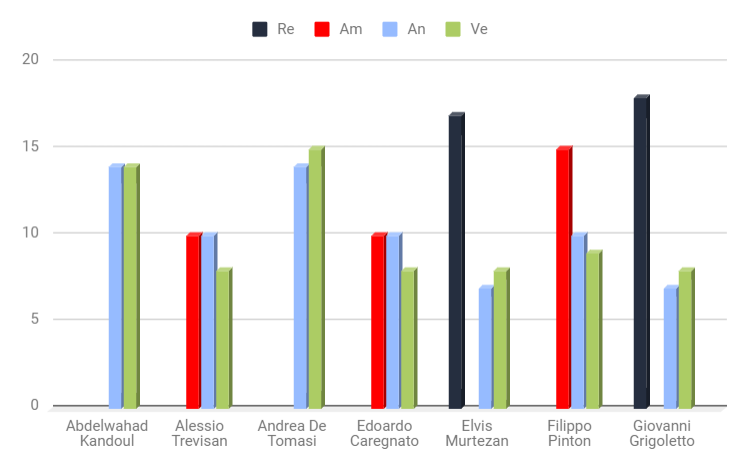
\includegraphics[width=1\textwidth]{./src/Preventivo/src/img/IstoAnalisi.png}
%\begin{center}
%	\pgfplotsset{width=15.4cm, height=8.5cm}
%	\begin{tikzpicture}
%		\begin{axis}[
%			ybar stacked,
%			bar width=20pt,
%			legend style={
%				at={(0.5,-0.15)},
%				anchor=north,
%				legend columns=-1
%			},
%			symbolic x coords={Abdelwahad, Alessio, Andrea, Edoardo, Elvis, Filippo, Giovanni},
%			xtick=data
%		]
%			\legend{Responsabile, Amministratore, Analista, Progettista, Programmatore, Verificatore}
			% Responsabile
%			\addplot [ybar, fill=blue] coordinates {\ColonnaIstogramma{0}{0}{0}{0}{17}{0}{18}};
			% Amministratore
%			\addplot [ybar, fill=yellow] coordinates {\ColonnaIstogramma{0}{10}{0}{10}{0}{15}{0}};
			% Analista
%			\addplot [ybar, fill=red] coordinates {\ColonnaIstogramma{14}{10}{14}{10}{7}{10}{7}};
			% Progettista
%			\addplot [ybar, fill=green] coordinates {\ColonnaIstogramma{0}{0}{0}{0}{0}{0}{0}};
			% Programmatore
%			\addplot [ybar, fill=pink] coordinates {\ColonnaIstogramma{0}{0}{0}{0}{0}{0}{0}};
			% Verificatore
%			\addplot [ybar, fill=orange] coordinates {\ColonnaIstogramma{14}{8}{15}{8}{8}{9}{8}};
%		\end{axis}
%	\end{tikzpicture}
%\end{center}
\clearpage

\subsubsection{Costo risultante}
La seguente tabella rappresenta per ogni ruolo le ore totali investite ed il corrispondente costo in euro:
{
\rowcolors{2}{\evenRowColor}{\oddRowColor}
\renewcommand{\arraystretch}{2}
\begin{longtable}{ C{3cm} C{2cm} C{4cm}}
\caption{Tabella del costo risultante di analisi}\\
\rowcolor{\primaryColor}

\textcolor{\secondaryColor}{\textbf{Ruolo}} & 
\textcolor{\secondaryColor}{\textbf{Totale ore}} & 
\textcolor{\secondaryColor}{\textbf{Costo ruolo (in \euro{})}}\\	
\endhead

Responsabile    &  35 &  1050 \\
Amministratore  &  35 &  700 \\
Analista        &  71 & 1775 \\
Progettista     &   - &  - \\
Programmatore   &   - &  - \\
Verificatore    &  70 & 1050 \\
\textbf{Totale} & 211 & 4575 \\
		
\end{longtable}
}

\vskip 30pt %spazio verticale
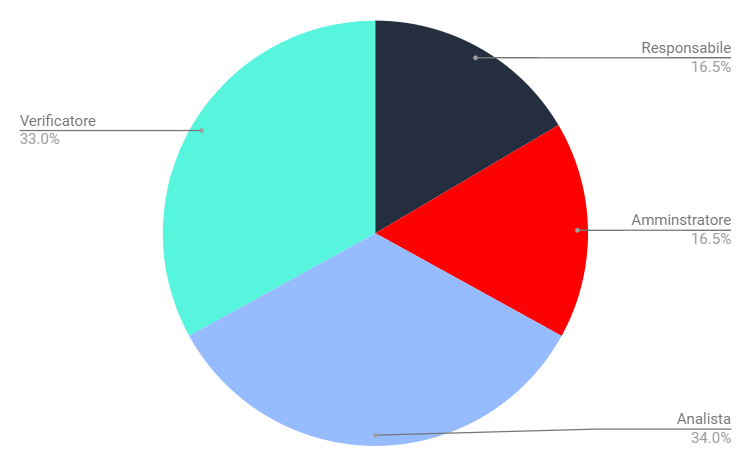
\includegraphics[width=1\textwidth]{./src/Preventivo/src/img/TortaAnalisi.png}
%La quantità di ore totali investite per ciascun ruolo viene rappresentata nel seguente areogramma:
%\begin{center}
%	\pgfplotsset{width=17cm, height=8.5cm}
%	\begin{tikzpicture}
%		\pie[rotate = 180, color={blue, yellow, red, orange}] {
%			17/Responsabile,
%			17/Amministratore,
%			33/Analista,
%			33/Verificatore
%		}
%	\end{tikzpicture}
%\end{center}
\subsection{Analisi dei Requisiti}
\subsubsection{Bilancio}
Il bilancio della fase di Analisi è positivo, ovvero il gruppo ha impiegato meno ore di quelle anticipate, quindi il costo finale della fase di Analisi è minore dell'aspettativa calcolata in precedenza.\\
La seguente tabella illustra la differenza oraria ed economica rilevata a posteriori.

{
\rowcolors{2}{\evenRowColor}{\oddRowColor}
\renewcommand{\arraystretch}{2}
\begin{longtable}[h]{ C{2.5cm} C{2.5cm} C{2.5cm} C{2.5cm} C{1.5cm} C{2.5cm}}
\caption{Tabella del costo complessivo per ruolo}\\
\rowcolor{\primaryColor}

\textcolor{\secondaryColor}{\textbf{Ruolo}} & 
\textcolor{\secondaryColor}{\textbf{Ore preventivate}} & 
\textcolor{\secondaryColor}{\textbf{Variazione oraria}} & 
\textcolor{\secondaryColor}{\textbf{Costo preventivato (in \euro{})}} & 
\textcolor{\secondaryColor}{\textbf{Costo effettivo (in \euro{})}} & 
\textcolor{\secondaryColor}{\textbf{Variazione di costo (in \euro{})}}\\	
	
Responsabile    &  35 & 0 & 1050 & 1050 &  0 \\
Amministratore  &  35 & 0 & 700 & 700 & 0 \\
Analista        & 71 & 4 & 1775 & 1425 & 350 \\
Progettista     &   0 &   0 &    0 &  0 & 0 \\
Programmatore   &   0 &   0 &    0 &  0 & 0 \\
Verificatore    &  70 &  5 & 900 &  & 75 \\
\textbf{Totale} & 211 & 202 & 4575 & 4400 & 175 \\	

\end{longtable}
}

\subsubsection{Conclusioni}
Come riportato dalla tabella, il bilancio risulta essere positivo per i seguenti motivi:
\begin{itemize}
	\item \textbf{Responsabile}: {i componenti designati a questo ruolo in questa fase a fare i responsabili non avevano esperienza è quindi le ore preventivate hanno tenuto conto di questo; }
	\item \textbf{Amministratore}: {uno dei componenti del gruppo aveva già esperienza in merito a vari strumenti e tecnologie utilizzabili per migliorare la produttività del gruppo,ma è stato tenuto 
	conto del inesperienza di alcuni componenti del team in questo ruolo;}
	\item \textbf{Analista}: {è in linea col preventivo}
	\item \textbf{Verificatore}: {lo scostamento è in linea con il preventivo all'incirca come quelle dell'analista che sono molto legate tra di loro in questa fase.}
\end{itemize}

\subsubsection{Ragionamento sugli scostamenti}
La suddivisione a stadi di una fase permette di migliorare la produttività del team, visto che viene effettuato un check intermedio alla fine di uno stadio:
\begin{itemize}
	\item Dai \textbf{verificatori}, che validano i deliverables relativi a quello stadio;
	\item E dal \textbf{responsabile}, che verifica la presenza di eventuali problematiche.
\end{itemize}
Questo fa presupporre che anche i futuri scostamenti siano abbastanza in linea con quello preventivato.
\subsubsection{Preventivo a finire}
Il costo effettivo di questa prima fase non ha influenza sul preventivo in quanto esso si basa solamente sui costi preventivati nelle fasi successive di Progettazione, Codifica, Collaudo.\\
Ciò non toglie che ragionando sugli scostamenti, il gruppo deve prestare qualche attenzione in più sulla pianificazione oraria, ma nel complesso il team pianifica e lavora bene.
